\documentclass{beamer}
\usepackage{risk201}

\setchapter{2}

% Chapter-specific diagram shortcuts
% Timeline 0, 1, ..., 4, 5 used in the examples of Section 2.1
\newcommand{\examtimeline}[3]{%
  \cftimeline{7}{0/0/{}, 1.5/1/{#1}, 4.5/4/{#2}, 6.5/5/{#3}}{\node at (3,-0.4) {$\ldots$};}%
}


\title{RISK 201: Equivalence Equations}

\begin{document}
\maketitle

%======================================================================
\section{Equations of value}
%======================================================================

\begin{frame}{2.1 Equations of value}

Some observations:
\begin{itemize}
\item Money has time value.
\item We need \textbf{dates} attached to each cash flow to be able to make comparisons.
\item If we are indifferent between two options, we say the cash flows are \textbf{equivalent}. Formally:
\end{itemize}

\begin{center}
\blue{$X$ due on a given date is equivalent \\
at a given compound interest rate $i$ \\
to an amount $Y$ due $n$ periods later \\[1ex]
if $Y = X(1+i)^n$}
\end{center}

\end{frame}

\begin{frame}{Transitivity under compound interest}

\begin{center}
At a given compound interest rate, \\
if \blue{$X$} is equivalent to \orange{$Y$}, and \orange{$Y$} is equivalent to $Z$, \\
then \blue{$X$} is equivalent to $Z$.

\bigskip
\cftimeline{8}{0/0/{}, 2.5/t_1/{\blue{$X$}}, 5.5/t_2/{\orange{$Y$}}, 7.5/t_3/{$Z$}}{}

\begin{align*}
\orange{Y} &= \blue{X}(1+i)^{t_2-t_1} \\
Z &= \orange{Y}(1+i)^{t_3-t_2}
\end{align*}
\[
\Rightarrow Z = \blue{X}(1+i)^{t_2-t_1}(1+i)^{t_3-t_2} = \blue{X}(1+i)^{t_3-t_1}
\]
\end{center}

\end{frame}

\begin{frame}{Sets of cash flows}

Some more observations:
\begin{itemize}
\item Often, we care about a \blue{\textbf{set of dated cash flows}} and want to know their combined value.
\item Adding up values in the set makes no sense if they are at different dates.
\item Solution: replace the dated cash flows in the set with equivalent cash flows all due on the \orange{\textbf{same}} date, THEN add them up $\to$ \blue{\textbf{dated value of the set}}
\item The common date is called the \blue{\textbf{valuation date}}, or \blue{\textbf{comparison date}}, or \blue{\textbf{focal date}}.
\end{itemize}

\end{frame}

\begin{frame}{Example 2.1}

An investment guarantees to pay \$400 in 1 year, \$200 in 4 years, and \$100 in 5 years. What is the value of this investment today if $i = 5\%$?

\begin{center}
\examtimeline{400}{200}{100}
\end{center}

\vfill
\end{frame}

\begin{frame}{Example 2.1, continued}

What is the value of this investment a year from now? Four years from now? 10 years from now?

\begin{center}
\examtimeline{400}{200}{100}
\end{center}

\vfill
\end{frame}

\begin{frame}{Keeping track of cash in and out}

\begin{itemize}
\item Some of the cash flows in our set may be income, some may be outlays (aka outgo):
  \begin{itemize}
  \item A loan vs the repayments
  \item An initial investment vs its returns
  \end{itemize}
\item Attach opposite signs to cash income and outgo $\to$ dated \blue{\textbf{directional}} cash flows
\end{itemize}

\end{frame}

\begin{frame}{Example 2.2}

An investment \blue{guarantees to pay} \$400 in 1 year, and \$100 in 5 years, but \orange{requires an additional cash injection} of \$200 after 4 years. What is the value of this investment today if $i = 5\%$?

\begin{center}
\examtimeline{\blue{400}}{\orange{$-200$}}{\blue{100}}
\end{center}

\vfill
\end{frame}

\begin{frame}{Example 2.2, continued}

\begin{center}
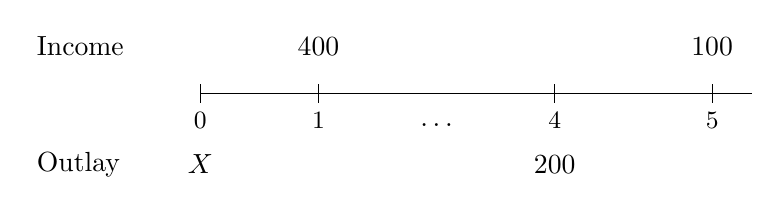
\begin{tikzpicture}
  \node[anchor=west] at (-2.2,0.6) {\blue{Income}};
  \node[anchor=west] at (-2.2,-0.9) {\orange{Outlay}};
  \draw (0,0) -- (7,0);
  \foreach \x/\lab in {0/0, 1.5/1, 4.5/4, 6.5/5} {
    \draw (\x,0.12) -- (\x,-0.12);
    \node[below] at (\x,-0.12) {\small $\lab$};
  }
  \node at (3,-0.4) {$\ldots$};
  \node at (1.5,0.6) {\blue{400}};
  \node at (6.5,0.6) {\blue{100}};
  \node at (0,-0.9) {\orange{$X$}};
  \node at (4.5,-0.9) {\orange{200}};
\end{tikzpicture}
\end{center}

\vfill
\begin{center}
dated value of \blue{income} $=$ dated value of \orange{outlay} \\
on a common valuation date, at a given rate $i$
\end{center}

\end{frame}

\begin{frame}{Simple interest \& simple discount}

\begin{itemize}
\item \textbf{Only} compound interest has the transitive property for accumulation!
\item Under simple interest (or simple discount), if \blue{$X$} is equivalent to \orange{$Y$}, and \orange{$Y$} is equivalent to $Z$, then \blue{$X$} is NOT equivalent to $Z$.
\end{itemize}

\begin{center}
\cftimeline{8}{0/0/{}, 2.5/t_1/{\blue{$X$}}, 5.5/t_2/{\orange{$Y$}}, 7.5/t_3/{$Z$}}{}

\[
\orange{Y} = \blue{X}\bigl(1+(t_2-t_1)i\bigr), \qquad Z = \orange{Y}\bigl(1+(t_3-t_2)i\bigr),
\]
\vspace{-3ex}
\begin{align*}
\Rightarrow Z &= \blue{X}\bigl(1+(t_2-t_1)i\bigr)\bigl(1+(t_3-t_2)i\bigr) \\
&\neq \blue{X}\bigl(1+(t_3-t_1)i\bigr)!
\end{align*}
\end{center}

\end{frame}

\begin{frame}{Types of problems}

\footnotesize
\renewcommand{\arraystretch}{1.2}
\begin{tabular}{@{}>{\raggedright\arraybackslash}p{0.21\textwidth}>{\raggedright\arraybackslash}p{0.18\textwidth}p{0.38\textwidth}p{0.11\textwidth}@{}}
\toprule
\textbf{Given} & \textbf{Find} & \textbf{Technique} & \textbf{Example} \\
\midrule
Two or more streams of payments, interest rate, times of payments
& Preferred stream of payments
& \vspace{-2ex}\begin{itemize}
  \item Choose valn date
  \item Value all cash flows
  \item Compare
  \end{itemize}
& 2.3 \\
\midrule
Amounts of some payments, interest rate, times of payments
& Missing payment(s) that make cash flows equivalent
& \vspace{-2ex}\begin{itemize}
  \item Choose valn date
  \item Equate value of all cash flows at that date
  \item Solve for missing payment(s)
  \end{itemize}
& 2.4 \\
\bottomrule
\end{tabular}

\end{frame}

\begin{frame}{Example 2.3 (Brown \& Kopp 1.10.A17)}

A piece of land can be purchased by paying \$500,000 cash or \$200,000 down and equal payments of \$200,000 at the end of two and four years respectively. To pay cash, the buyer would have to withdraw money from an investment earning interest at $i^{(2)} = 8\%$. Which option is better and by how much?

\vfill
\end{frame}

\begin{frame}{Example 2.4 (Brown \& Kopp 2.1.A15)}

Mrs.\ Singh borrows \$3000, due with interest at $i^{(12)} = 9\%$ in 2 years. The lender agrees to let Mrs.\ Singh repay the loan with a payment of \$1000 in 6 months, \$1500 in 12 months, and \$$X$ in 30 months. If money is worth $i^{(2)} = 6\%$, what is the value of $X$?

\vfill
\end{frame}

%======================================================================
\section{Determining rate and time}
%======================================================================

\begin{frame}{2.2 Determining rate and time}

\small
\renewcommand{\arraystretch}{1.2}
\begin{tabular}{@{}>{\raggedright\arraybackslash}p{0.24\textwidth}>{\raggedright\arraybackslash}p{0.26\textwidth}p{0.42\textwidth}@{}}
\toprule
\textbf{Given} & \textbf{Find} & \textbf{Technique} \\
\midrule
Amounts of all payments, interest rate
& Time of payment that makes cash flows equivalent
& \vspace{-2ex}\begin{itemize}
  \item Choose valn date
  \item Equate value of all cash flows at that date
  \item Solve for $t$
  \end{itemize} \\
\midrule
Amounts of all payments, times of payments
& Interest rate that makes cash flows equivalent
& \vspace{-2ex}\begin{itemize}
  \item Choose valn date
  \item Equate value of all cash flows at that date
  \item Solve for $i$
  \end{itemize} \\
\bottomrule
\end{tabular}

\end{frame}

\begin{frame}{Finding the interest rate}

\textbf{Algorithm}
\begin{enumerate}
\item Consider the compounding period
\item Write the equation of value in terms of $j$, the effective rate per compounding period
\item Solve for $j$
\item Convert to whatever effective or nominal rate is required.
\end{enumerate}

\end{frame}

\begin{frame}{Finding the interest rate}

\textbf{On your financial calculator}
\begin{enumerate}
\item N = the number of compounding periods
\item PV = $-$ present value
\item FV = future value
\item PMT = periodic payments (zero in this context)
\item CPT I/Y (interest rate per compounding period)
\end{enumerate}

\bigskip
NOTE: The rate will be given as a \%, not a decimal

\end{frame}

\begin{frame}{Example 2.5 (Brown \& Kopp 2.2.A10)}

If an investment grows by 50\% in 4 years, what rate of interest $i^{(4)}$ is being earned?

\vfill
\end{frame}

\begin{frame}{Example 2.5, continued}

\textbf{On your financial calculator}
\begin{enumerate}
\item N = 16
\item PV = $-100$
\item FV = 150
\item PMT = 0
\item CPT I/Y
\end{enumerate}

\vfill
\end{frame}

\begin{frame}{Finding the time}

\textbf{Algorithm}
\begin{enumerate}
\item Consider the compounding period
\item Write the equation of value in terms of $j$, the effective rate per compounding period (if annual, use $i$)
\item Solve for the time (in the exponent) by taking logs of both sides
\end{enumerate}

\end{frame}

\begin{frame}{Finding the time}

\textbf{On your financial calculator}
\begin{enumerate}
\item PV = $-$ present value
\item FV = future value
\item PMT = periodic payments (zero)
\item I/Y = interest rate per compounding period (\%)
\item CPT N (the number of compounding periods)
\end{enumerate}

\end{frame}

\begin{frame}{Example 2.6}

How long does an investment take to double at a given rate of compound interest?

\vfill
\begin{flushright}
\begin{tabular}{cc}
\toprule
$i$ & $t$ \\
\midrule
2\% & 35.00 \\
4\% & 17.67 \\
6\% & 11.90 \\
8\% & 9.00 \\
10\% & 7.27 \\
\bottomrule
\end{tabular}
\end{flushright}

\end{frame}

\begin{frame}{Rule of 72}

\textbf{On your financial calculator}
\begin{enumerate}
\item PV = $-100$
\item FV = 200
\item PMT = 0
\item I/Y = 2, 4, 6, 8, 10, \ldots
\item CPT N
\end{enumerate}

\vfill
\end{frame}

\begin{frame}{Example 2.7}

You are offered \$100 now plus \$100 in a year, or \$400 at a later time. If the two options are equivalent at $i = 12\%$ when would you receive the \$400?

\vfill
\end{frame}

%======================================================================
\section{Inflation \& real rates of interest}
%======================================================================

\begin{frame}{2.3 Inflation \& real rates of interest}

Inflation refers to the general increase in the price of goods over time.

\begin{center}
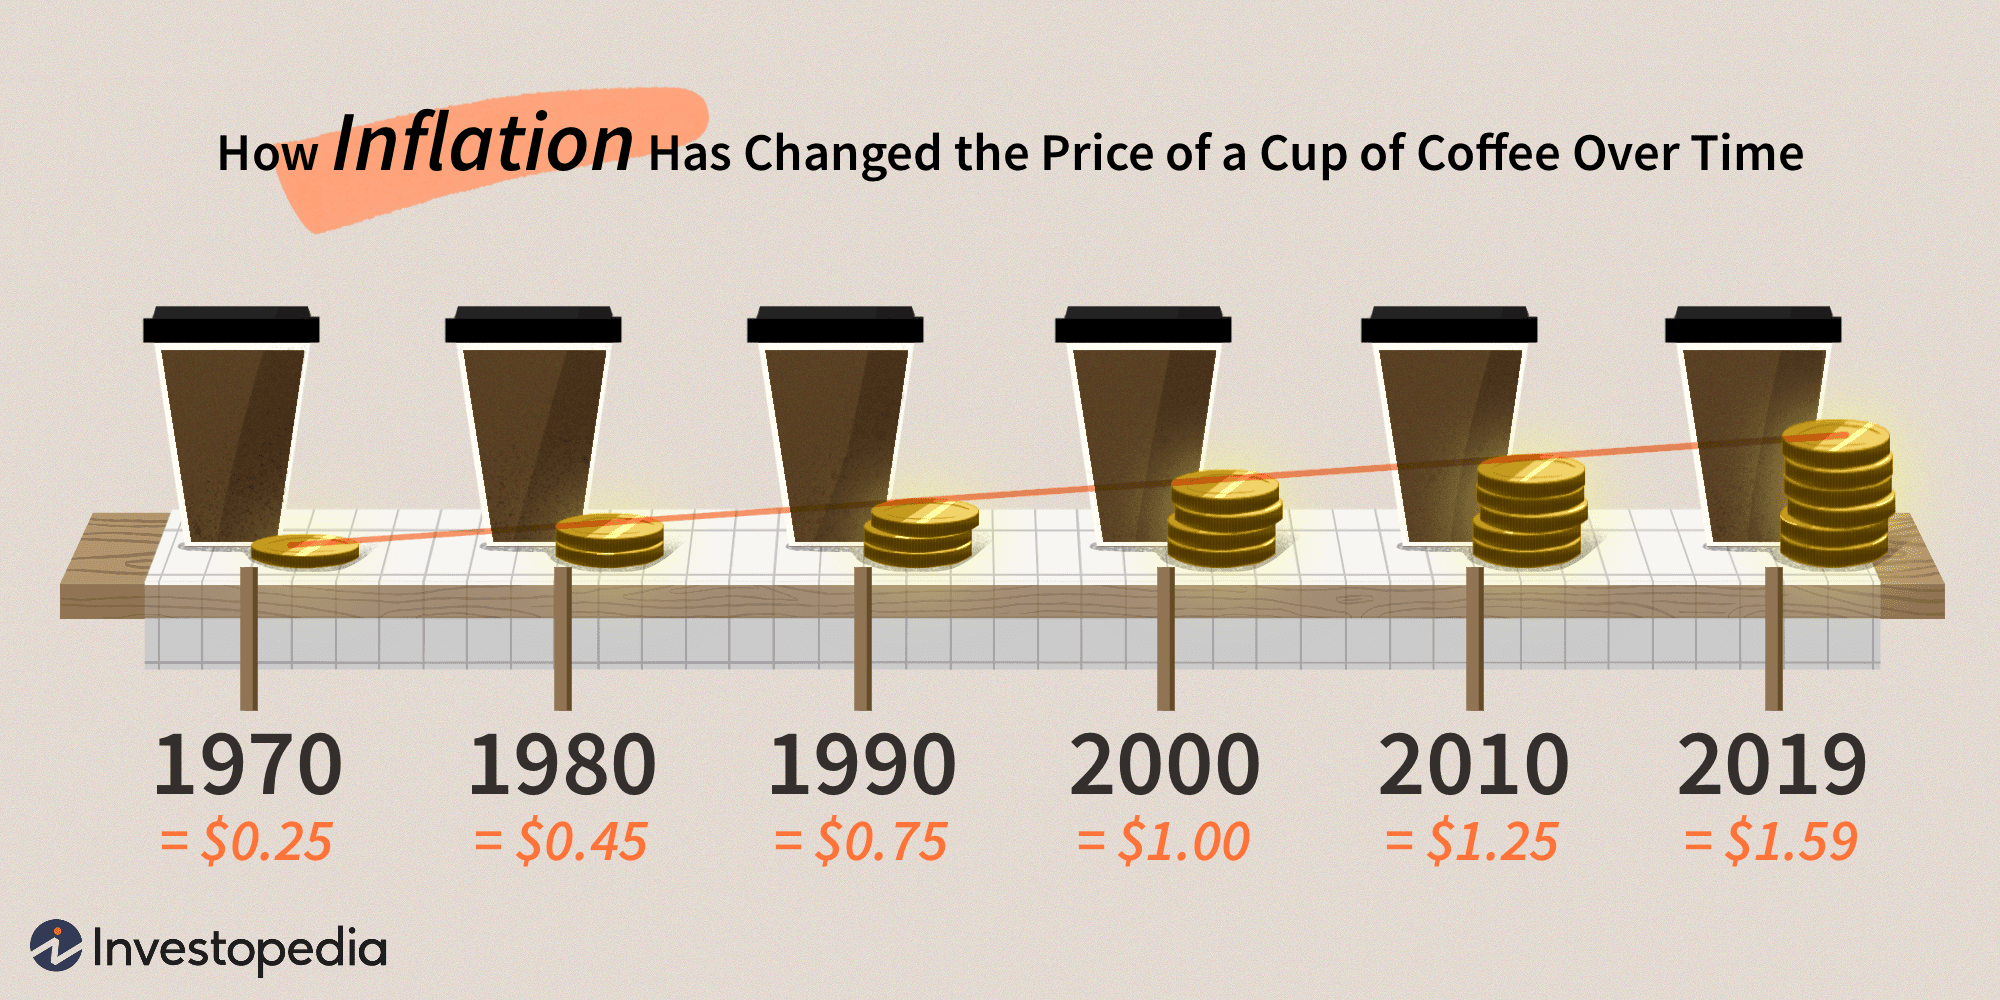
\includegraphics[height=0.5\textheight]{figures/ch2_coffee_prices.png}
\end{center}

Inflation erodes the purchasing power of money.

\end{frame}

\begin{frame}{Why do we have inflation?}

\begin{center}
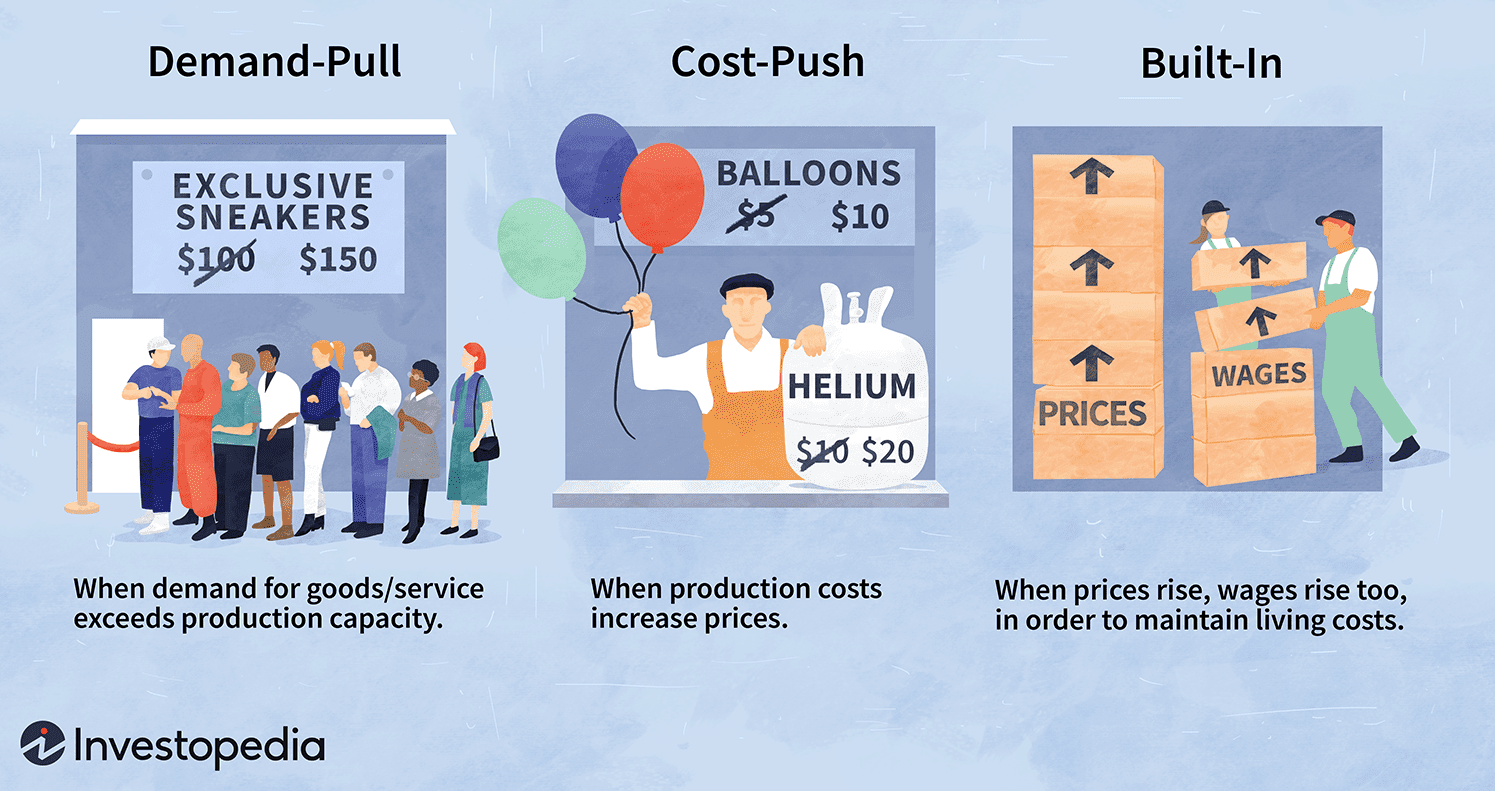
\includegraphics[width=\textwidth]{figures/ch2_inflation_causes.png}
\end{center}

\end{frame}

\begin{frame}{Inflation rate}

The inflation rate is the (annualized) rate of change in the prices of consumer goods.

\bigskip
\begin{tabular}{@{}ll}
Price of milk (4L) in Dec 2021: & \$5.07 \\
Price of milk (4L) in Nov 2022: & \$6.27 \\
\textcolor{red}{Price of milk (4L) in Nov 2024:} & \textcolor{red}{\$6.63!}
\end{tabular}

\bigskip
For specific goods, see \href{https://www150.statcan.gc.ca/t1/tbl1/en/tv.action?pid=1810024501}{\blue{\underline{Statistics Canada}}}.

\end{frame}

\begin{frame}{The Consumer Price Index (CPI)}

\begin{itemize}
\item Inflation is measured by reference to an index that captures the average price of a specified basket of goods at different points in time.
\item Inflation can be specific to a \href{https://www150.statcan.gc.ca/t1/tbl1/en/tv.action?pid=1810000501}{\blue{\underline{segment or sector of the economy}}}.
\item A widely used index is the Consumer Price Index (CPI).
\item Statistics Canada constructs and estimates the Canadian CPI. See \href{https://www23.statcan.gc.ca/imdb/p2SV.pl?Function=getSurvey&SDDS=2301&lang=en&db=imdb&adm=8&dis=2}{\blue{\underline{here}}} to learn how.
\item For information about the CPI in 2021, see \href{https://www150.statcan.gc.ca/n1/pub/11-627-m/11-627-m2022004-eng.htm}{\blue{\underline{here}}}.
\end{itemize}

\end{frame}

\begin{frame}{Hyperinflation}

\begin{itemize}
\item Hyperinflation refers to a very rapid increase in the price of goods and services: over 50\% per month (Cagan, 1956)
\item Hanke and Krus (2013) compiled a list of 56 hyperinflation events from around the world.
\item The highest level of inflation occurred in Hungary
  \begin{itemize}
  \item monthly inflation rate (July 1946): $4.19 \times 10^{16}\%$!
  \item equivalent daily inflation rate: 207\%
  \item time required for prices to double: 15 hours\ldots
  \end{itemize}
\end{itemize}

\end{frame}

\begin{frame}{Hyperinflation}

\begin{center}
\begin{tikzpicture}
  \node[anchor=north west, inner sep=0] (hu) at (0,0)
    {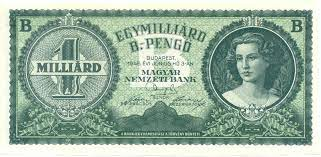
\includegraphics[width=0.47\textwidth]{figures/ch2_hungary_banknote.png}};
  \node[anchor=north west, inner sep=0] (zw) at (0,-2.9)
    {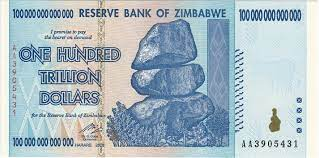
\includegraphics[width=0.47\textwidth]{figures/ch2_zimbabwe_banknote.png}};
  \node[anchor=north east, inner sep=0] (ve) at (\textwidth,-2.1)
    {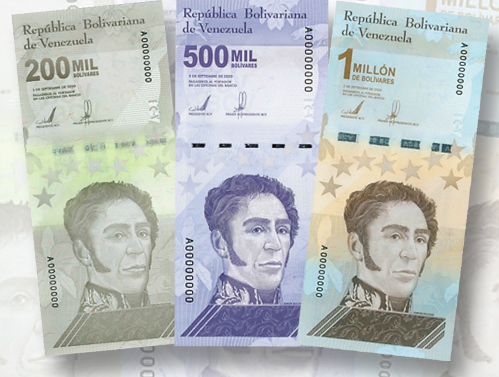
\includegraphics[width=0.42\textwidth]{figures/ch2_venezuela_banknotes.png}};
  \draw[-latex, line width=3pt, blue!70] (0.565\textwidth,-1.0) -- (0.49\textwidth,-1.0);
  \node[anchor=west, align=center, font=\scriptsize] at (0.58\textwidth,-1.0)
    {1 billion trillion = \\ 1,000,000,000,000,000,000,000};
\end{tikzpicture}
\end{center}

\end{frame}

\begin{frame}{Inflation and interest rates}

\blue{\textbf{Inflation counteracts investment growth.}}

\underline{Example 2.8:} You have \$1000 today and inflation is 5\% per year. What is the relative purchasing power of your \$1000 after one year (if not invested)?

\vfill
You invest your \$1000 at $i = 12\%$. What is the relative purchasing power of the accumulated value at the end of the year?

\vfill
\end{frame}

\begin{frame}{The real interest rate}

\underline{Example 2.8, continued:}

What is the rate of interest earned during the year, after adjusting for inflation? \textcolor{cyan!70!blue}{6.666\%}

\vfill
We call this the \blue{\textbf{real/net/inflation-adjusted rate of interest}} and denote it by $i_{real}$.
\[
i_{real} = \frac{1+i}{1+r} - 1
\]

\end{frame}

\begin{frame}{Another ``nominal'' interest rate}

The interest rate that has not been adjusted for inflation is called the \blue{\textbf{nominal interest rate}}.

\bigskip
Note that ``nominal'' here means something different than in Section 1.7!

\end{frame}

\begin{frame}{Example 2.9}

Amy expects to receive four annual scholarship payments. The first payment (due now) is \$10,000. Each successive payment is adjusted for inflation so that in real terms the payments remain level. Inflation is 3\% per year and the effective interest rate is 6\% a year. Find the present value of Amy's scholarship.

\vfill
\end{frame}

\begin{frame}{Finding the present value}

\textbf{On your financial calculator}
\begin{enumerate}
\item N = the number of compounding periods
\item I/Y (\textcolor{red}{real} interest rate per compounding period)
\item FV = future value (how much?)
\item PMT = periodic payments
\item CPT PV = $-$ present value
\end{enumerate}

\end{frame}

\begin{frame}{Negative real rates of interest}

When inflation $(r)$ is higher than the nominal interest rate $(i)$, the real rate of interest is negative. When this happens, there is an incentive to borrow.

\bigskip
\fbox{\parbox{0.95\textwidth}{%
\underline{Example 2.10:} You borrow \$1000 for one year. Interest is charged at 2\% and inflation is 4\%. How much do you have to pay back at the end of the year

\medskip
(a) in nominal terms?

\vspace{2em}
(b) in real terms?

\vspace{2em}
}}

\end{frame}

\begin{frame}{References}

\small
\begin{itemize}
\item[] Cagan, P. (1956). `The monetary dynamics of hyperinflation', in Friedman, M. (ed.) \textit{Studies in the Quantity Theory of Money.} Chicago, IL: University of Chicago Press.
\item[] Hanke, S.H. and Krus, N. (2013) `World hyperinflations', in Parker, R.E. and Whaples, R.M. (eds.) In \textit{Routledge Handbook of Major Events in Economic History.} Routledge.
\end{itemize}

\end{frame}

\end{document}
